\documentclass[10pt,twocolumn]{witseiepaper}

%
% All KJN's macros and goodies (some shameless borrowing from SPL)
\usepackage{KJN}
\usepackage{subcaption}
\usepackage{listings}
\usepackage{amsmath}
\usepackage{epstopdf}
\usepackage{xcolor}
\usepackage{textcomp}
\usepackage{listings}
\usepackage{alltt}
\usepackage{matlab-prettifier}
\usepackage{graphicx}
\usepackage{changes}
\usepackage{makecell}
\usepackage{verbatim}
\usepackage{algorithm,algpseudocode}
\usepackage{balance}
\usepackage{pdfpages}
\usepackage{longtable}
\usepackage{tikz} % for drawing stuff
\usetikzlibrary{positioning} % for relative coordinates
\usepackage{color} %red, green, blue, yellow, cyan, magenta, black, white
\definecolor{mygreen}{RGB}{28,172,0} % color values Red, Green, Blue
\definecolor{mylilas}{RGB}{170,55,241}
%\usepackage{flafter}

\lstset{language=Matlab, % Set colour for matlab code
	breaklines=true,%
	morekeywords={matlab2tikz},
	keywordstyle=\color{blue},%
	morekeywords=[2]{1}, keywordstyle=[2]{\color{black}},
	identifierstyle=\color{black},%
	stringstyle=\color{mylilas},
	commentstyle=\color{mygreen},%
	showstringspaces=false,%without this there will be a symbol in the places where there is a space
	numbers=left,%
	numberstyle={\tiny \color{black}},% size of the numbers
	numbersep=9pt, % this defines how far the numbers are from the text
	emph=[1]{for,end,break},emphstyle=[1]\color{red}, %some words to emphasise
	%emph=[2]{word1,word2}, emphstyle=[2]{style},    
}
\usepackage{lmodern}
\newcommand*{\escape}[1]{\texttt{\textbackslash#1}}

%
% PDF Info
%
\ifpdf
\pdfinfo{
/Title (FILE TRANSFER APPLICATION)
/Author (KJ Butkow, Jared Ping)
/CreationDate (D:201803151731)
/ModDate (D:200510121530)
/Subject (FILE TRANSFER APPLICATION)
/Keywords ()
}
\fi

%%%%%%%%%%%%%%%%%%%%%%%%%%%%%%%%%%%%%%%%%%%%%%%%%%%%%%%%%%%%%%%%%%%%%%%%%%%%%%%
\begin{document}


\title{FILE TRANSFER APPLICATION  \\ ELEN4017 Project Report}

\author{Kayla-Jade Butkow (714227) and Jared Ping (704447)
\thanks{School of Electrical \& Information Engineering, University of the
Witwatersrand, Private Bag 3, 2050, Johannesburg, South Africa}
}


%%%%%%%%%%%%%%%%%%%%%%%%%%%%%%%%%%%%%%%%%%%%%%%%%%%%%%%%%%%%%%%%%%%%%%%%%%%%%%%
%
\abstract{This paper presents the design, implementation and testing of a File Transfer Application, consisting of a server and a graphical user interface client. The developed system follows the guidelines set out in RFC 959, and exceeds the required minimum specifications. Wireshark was used to obtain results, and from the collected packets, it was clear that the request and response messages follow the correct order. The implemented server is able to interact with a standard FTP client, and the client is able to interact with a standard FTP server. The server is also able to handle multiple simultaneous control connections and data connections. Future reccomendations include the implementation of multiple transmission modes and file structures.}

\keywords{client, file transfer protocol, server, Wireshark}

\maketitle
\thispagestyle{empty}
\pagestyle{plain}
\setcounter{page}{1}

%%%%%%%%%%%%%%%%%%%%%%%%%%%%%%%%%%%%%%%%%%%%%%%%%%%%%%%%%%%%%%%%%%%%%%%%%%%%%%%
%
\section{INTRODUCTION}
The File Transfer Protocol (FTP) is essential in the implementation of a File Transfer Application. The File Transfer Protocol allows for the transfer of files between two end systems \cite{kurose}. The FTP protocol runs on top of TCP and, uniquely, makes use of two TCP connections: a control connection and a data connection \cite{kurose}. The data connection is non-persistent, and is created when the transfer of data is required \cite{kurose}. A File Transfer Application consists of an FTP server and an FTP client. This report presents the design, implementation and testing of a File Transfer Application, including an overview of the system, details of the implemented code, results and a critical analysis of the system. The division of labour between group members is also discussed.

\section{SYSTEM OVERVIEW}
The implemented system follows the guidelines set out in RFC 959 - File Transfer Protocol (FTP) \cite{rfc}. This document specifies the minimum required FTP implementation as well as the full list of FTP commands and replies.

\subsection{FTP Server}
The FTP server runs from the user's local host and allows users to connect through a locally hosted FTP client, as well as through clients on the same network. The server facilitates the storage of files and a user management system. The server is capable of running on any Unix based system.

The server's user management system functions by requesting users to authenticate themselves upon connecting to the server. This information is used to provide each user with their own maintained file repository. The repository implementation allows the user to only access their files and prevents users from being aware of other user repositories, providing a secure and user-tailored experience. Unauthenticated users will be unable to perform any modification operations such as uploading and deleting files.

The server has been created in accordance with the RFC 959 standards to allow for compatibility with standard FTP clients, allowing users to connect to the server from a range of clients. An extensive number of RFC commands have been implemented to provide improved compatibility and functionality for FTP clients which utilise the additional commands. A server logger has also been implemented to track client requests in real-time for server monitoring and debugging capabilities.

Multi-threading has been utilised in the development of the server to facilitate simultaneous client connections. This supports both connection and server request operations, allowing for multiple users to connect, browse directories, and upload and download files concurrently.

\subsubsection*{Unimplemented Features:}
The file structure type of the server is defaulted to the file structure, with the page and record structures not being implemented due to complexity and time overhead. The data transmission mode of the server is defaulted to the stream mode, with the block and compression modes not being implemented due to complexity and time overhead. The default structure type and data transmission mode is set to be the file structure and stream mode respectively for any FTP application in accordance with RFC 959, thus no client compatibility issues will be encountered \cite{rfc}. The lack of compression data transmission mode results in a lower available bandwidth for very large network transmissions \cite{rfc}.

\subsection{FTP Client}
The FTP client runs from the user's local host and allows the user to interact with the FTP server in order to transfer files. In order to improve user experience, a client with a graphical user interface (GUI) was implemented. 

The client allows the user to specify the FTP server address that they wish to connect to, as well as the port that the server is running on. The user is also able to input their username and password for the FTP server they are connecting to.

Once the user has successfully connected to the FTP server, they are able to view their local file system as well as the remote file system within the client GUI. The user is also able to navigate both file systems. Once the required file is found, the user is able to upload the file to the remote server from the local file system, or download the file from the remote system to the local storage. When uploading a file, the file is saved to the currently selected directory on the server. If a directory has not been selected by the user, the file is saved to the home directory of the user's remote repository. Likewise, when the user is downloading a file, the file is saved to the current local folder, or if none is selected, to the user's home directory. On Mac OS X operating systems, this home directory is found at \textit{/Users/Username}. If a file is selected rather than a directory, the downloaded file is saved in the directory in which the selected file is found.

The user also has the ability to delete files or folders, as well as to recursively remove a folder and all of its contents. Finally, the user is able to create a folder on the server in the base directory of their choosing. If a file is selected rather than a base directory, the new directory is saved in the directory containing the selected file.

Once the client has finished using the FTP connection, they can disconnect from the server and connect to another server if they wish to.

\subsubsection*{Unimplemented Features:}
The feature to change the file structure from file to record or page was not implemented. This was not implemented since the implementation was complex and deemed unnecessary since any file can be transfered using the file structure. Furthermore, since the file structure is the default type, any server that the client wishes to interact with will be compatible with the file structure type \cite{rfc}. The client also does not allow the user the opportunity to change the transmission mode from stream to block or compression. Once again, since stream mode is the default mode, any FTP server must accept stream mode, meaning that implementation of the other types in unnecessary \cite{rfc}. The client also does not have implementation to allow the user to append data onto the end of an existing text file.

\section{COMMANDS AND REPLY CODES} \label{sec:commands}
There are five groups of reply codes determined by the first digit of the three digit code \cite{rfc}. These groups indicate whether the response is positive or negative and allow the client to make an informed decision as to its course of action.

The groups are as follows:
\begin{tabbing}
	\hspace{4em}\=\kill
1xx	\> Positive Preliminary Reply \\ 
2xx	\> Positive Completion Reply\\ 
3xx	\> Positive Intermediate reply \\ 
4xx	\> Transient Negative Completion reply \\ 
5xx	\> Permanent Negative Completion reply
\end{tabbing} 

At least one reply code from each group has been implemented. A list of the implemented commands and the reply codes is given in \tabref{tab:commands}. The table also contains a brief description of the purpose of each command.

\section{IMPLEMENTATION DETAILS}
The server and the client were both implemented using Python 3. On both systems, all communication sockets are created using the Python \texttt{socket} module \cite{socket}. The sending and receiving of messages are also performed using methods from this module. Interfacing with the operating system is performed using the \texttt{os} module \cite{os}. This module allows for the traversing of paths in the operating system, as well as for saving and opening files \cite{os}. 

Communication between the server and client is performed through the establishment of a TCP connection. This TCP connection acts as a control connection to transfer FTP commands and replies between the client and the server \cite{kurose}. When sending FTP commands to the server, the messages are formatted using the format in \figref{fig:commandformat}. In the figure, SP indicates a space and CRLF is the end of line sequence (\escape{r}\escape{n}). All communicated commands utilise \texttt{UTF-8} encoding to ensure communication compatibility.

\begin{figure}[h]
	\centering
	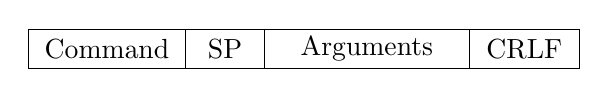
\begin{tikzpicture}
	\draw 
	(0,0) rectangle (2,-0.5) node[pos=.5] {Command}
	(2,0) rectangle (3, -0.5) node[pos=.5] {SP}
	(3,0) rectangle (5.6,-0.5) node[pos=.5] {Arguments}
	(5.6, 0) rectangle (7,-0.5) node[pos=.5] {CRLF}
	;
	\end{tikzpicture}
	\caption{FTP Command Format}
	\label{fig:commandformat}
\end{figure}

\subsection{Server}
In order to host client connections the server listens for any incoming connections which is established as a TCP connection between the two endpoints. A \texttt{serverListener()} function was created for this purpose with a socket configured to utilise the \texttt{SO\_REUSEADDR} argument which allows for active client connections to be maintained in the event of a sudden server restart. 

Each new incoming client connection was handled by binding the connection to a new thread to handle simultaneous connections. The instantiated thread waits for client transmission using the \texttt{recv()} function which is then decoded and the requested command is executed with a resulting response code that is encoding and sent back to the client using the \texttt{send()} function. The server utilises responses to provide the client with a result corresponding to the requested command. The aforementioned process is illustrated in \figref{fig:server}. These responses indicate command successes, errors, mode changes, and other relevant indicators. These response codes are described in Section~\ref{sec:commands}

\subsubsection*{Configuration:}
The server provides a range of configuration commands for clients to utilise based on how they are attempting to interact with the server. \texttt{PASV} specifies the server Data Transfer Process (DTP) to listen on a non-default data port to wait for a connection rather than initiate one upon receipt of a transfer command. \texttt{PORT} offers similar functionality however, the port is explicitly specified by the client. \texttt{MODE} specifies the data transfer method to be utilised by the server. \texttt{STRU} specifies the type of file structure to be used for representation of data by the server.

\subsubsection*{File browser:}
The server provides a range of file browser commands that offer the functionality of file browser commands in a terminal client. \texttt{PWD} prints the path of the current working directory. \texttt{CWD} allows for the client to change their current working directory path to another location. \texttt{CDUP} allows for the client to change the current working directory to the parent directory. \texttt{MKD} allows the client to make a directory in the current directory. \texttt{RMD} allows the client to remove the specified directory from the current directory. \texttt{DELE} allows the client to remove the specified directory from the current directory. \texttt{LIST} provides a list of content contained within the current working directory. Any deletion operation requires a user to be authenticated. A custom utility was created for \texttt{LIST} function to provide the client with as comprehensive information of the directory contents such as file permissions, file size and user group. \texttt{RNFR} and \texttt{RNTO} allows a client to rename a folder or file on the server.

\subsubsection*{File transfer:}
The server provides comprehensive functionality in its ability to handle file uploads and downloads. This begins with allowing clients to specify the file type through the \texttt{TYPE} command, allowing the differentiation between ASCII and binary file transfer. \texttt{RETR} and \texttt{STOR} facilitate a file being downloaded and uploaded respectively from the server. Furthermore, \texttt{APPE} allows a file to be uploaded with its content being appended to the file if it already exists on the server otherwise it server the same purpose as \texttt{STOR}. Any upload operation requires a user to be authenticated.

\subsubsection*{Miscellaneous:}
In addition to the existing server infrastructure, additional commands exist to improve the user experience. \texttt{NLST} returns only the names of content within a directory. \texttt{REST} specifies the server marker at which a file transfer is to be restarted. \texttt{SYST} returns the operating system of the server host. \texttt{HELP} returns the list of available server commands and their parameters to be supplied for successful use. \texttt{NOOP} functions as a connection testing command to ensure the client is still connected to the server. Finally, \texttt{QUIT} closes the client connection.

\subsection{Client}
In order to connect to the server, once the user has supplied the server address and port, a TCP connection is created between the server and the client. To communicate with the server, a \texttt{send()} function was created which takes in a string containing the FTP command, a space and the arguments. The end of line sequence is then appended to the string and the resulting string is transmitted to the server. The use of this function ensures that all messages sent to the server have the correct format. Once any control message has been sent to the server, the client receives the response, and decodes it into a string in the \texttt{receive()} function. To allow the user to see the responses from the server, all received responses are printed onto the GUI. In order to ensure that the \texttt{receive()} function is called after every message is sent, an \texttt{action()} function was created which calls the \texttt{send()} function and then the \texttt{receive()} function. 

Before uploading or downloading a file, the client sends a \texttt{PASV} command, which requests that the server creates a new data port and listens on that port for a connection from the client \cite{rfc}. As a response to the command, the server sends the client the IP address and port number of the new socket. The port number, which is a 16 bit number, is sent to the client as two eight bit numbers  \cite{rfc}. The port is therefore calculated by multiplying the first number (the most significant byte) by 256 and adding the result to the second number \cite{rfc}. Thereafter, the client connects to the port so that data can be transferred.

\subsubsection*{Uploading files:}
In order to upload a file, it is necessary to inform the server of whether an ASCII or binary file (image type) is being transmitted, so that the correct encoding can be used. In order to determine the type of the file to be uploaded, the \texttt{magic} module is used. The module determines the type of a file by classifying the file's headers \cite{magic}. If the type is found to be text, \texttt{TYPE A} is sent to the server. Otherwise, \texttt{TYPE I} is transmitted. Thereafter, a \texttt{STOR} command is sent to the server along with the full path of the file to be uploaded. Thereafter, the file is uploaded to the server. During the upload process, the file is divided up into chunks and each chunk transmitted to the server. A flow chart detailing the upload process is given in \figref{fig:upload}.

\subsubsection*{Downloading files:}
When downloading files, it is again necessary to specify the file type. Since the files lie on the server, the \texttt{magic} module could not be used to determine the file type. Rather, the file type was deduced from the file extension, using the \texttt{mimetypes} module. This file type is then compared to a list of ASCII file types, and if the file type is found in the list, \texttt{TYPE A} is sent to the server. Otherwise, \texttt{TYPE I} is transmitted. Once the file type has been sent, a \texttt{RETR} command is sent along with the full path of the file to be downloaded. A new file with the filename of the file to be downloaded is then opened. Chunks of data are received by the client and then written to the open file. Once no more data is received, the file is closed and the download is completed.

\subsubsection*{Deleting folders and files and making folders:}
The user is able to delete a file or folder on the remote system. They do so by selecting the file or folder and then pressing the \textit{Delete} button. The client then uses the method described below to determine whether the user is trying to delete a file or a folder. If a file is to be deleted, the \texttt{DELE} command is sent to the server. Likewise, for a folder, the \texttt{RMD} command is sent. Both of these commands are followed by the full path to the item to be deleted. The user is also able to create a folder by pressing the \textit{Create Directory} button. The pressing of this button prompts the user to input the name of the new folder. This folder is created using the \texttt{MKD} command, which is sent along with the path to the new directory.

\subsubsection*{Differentiating between files and folders:}
In many instances in the client, it is necessary to differentiate between a folder and a file on the server. Once such example of this is in deciding whether a \texttt{DELE} or \texttt{RMD} command should be sent, as described above. In order to differentiate, the response codes of the \texttt{CWD} command are used. If the response to a \texttt{CWD} command has a \texttt{550} code, it implies that the path points to a file and not a folder. If the response has a \texttt{250}, the path points to a folder. Thus, this method is used as a differentiator wherever one is needed.

\subsubsection*{GUI:}
The client was implemented as a GUI using the PyQt4 module. The GUI provided a simple user interface consisting of push buttons that allow the user to perform functions such as uploading and downloading files, and two file systems. The file systems of the server and client were created by taking the current path and creating a directory item for each of the directories in the path. The final directory is then populated with the folders and files contained in it. For the server file system, this information was obtained using the \texttt{PWD} and \texttt{LIST} commands. For the client file system, the information was obtained using the \texttt{walk} method of the \texttt{os} module. In order to change directories in the remote file system, a \texttt{CWD} command is sent along with the path to the directory of interest.

\section{DIVISION OF WORK}
Since the FTP server has two clear parts, the server and the client, the work was divided accordingly. Jared Ping wrote all of the code for the server, as well as the sections in the report pertaining to the server. Kayla-Jade Butkow wrote the code for the client, as the sections of the report related to the client. Kayla-Jade also wrote the section pertaining to the commands and reply codes and the introduction, while Jared detailed the structure of the code and wrote the conclusion. The critical analysis and results sections and the abstract were written by the partners together.

\section{RESULTS} \label{sec:results}
In order to test the system, it was necessary to test all of the implemented functionality on both the server and the client, as well as to test the interaction between the server and a standard FTP client, and between the client and a standard FTP server. This functionality was tested by performing actions on the various clients and then viewing the messages sent and responses receiving using Wireshark.

The most important functionality to be tested is the ability to log into the server, navigate through the remote file system and upload and download files. Furthermore, the ability to create a directory, delete files and directories and to log out of the server also needed to be tested. Tests of all of these functions were performed for each of the interactions mentioned below.

\subsection{Interaction between the implemented FTP server and client}

\figref{fig:gui} presents an image of the client interacting with the implemented server. From the image, it is clear that there is a unique repository for the user, and that the user is unable to navigate to other user's repositories.

\secref{sec:ourserverourclient} provides Wireshark excerpts of all of the implemented server client interactions. The excerpts prove that the client and server are compatible and that all of the required FTP functionality can be performed.

\figref{fig:multiple} shows that the server is able to handle multiple simultaneous connections. It can also be seen  from \figref{fig:multipleUpload} that simultaneous uploads and downloads from different users can be performed.

\subsection{Interaction between a standard FTP server and the implemented client}
In testing this interaction, it was necessary to ensure that the created client and the standard server were compatible and that all of the functionality implemented in the client functioned correctly when paired with a standard server. The server used can be found at \textit{ELEN4017.ug.eie.wits.ac.za}.

Wireshark screenshots indicating this functionality is given in \secref{sec:ourClientWitsServer}. From the images in \secref{sec:ourClientWitsServer}, it is evident that all functionality works as expected when paired with a standard FTP server.

\subsection{Interaction between the implemented FTP server and a standard FTP client}
The testing of this interaction is essential to ensure that the server can interact with clients other than the one created. This interaction was performed using the Mac OS X client, \textit{ForkLift}.

The results of the tests for this interaction are given in \secref{sec:ourserverstandardclient}. These screenshots again prove that the server is compatible with a standard FTP client.

\section{CRITICAL ANALYSIS}
An analysis of the successes and limitations of the implemented system is given below.

\subsection{Successes}
The system is a fully functional, stable and well implemented solution. As proven in \secref{sec:results}, it fulfils all of the requirements for a file transfer application, namely:
\begin{itemize}
	\item A client and a server that are able to meet all of the requirements of a minimal FTP implementation, as defined in \cite{rfc}, including server reply messages and error handling
	\item A client with a simple user interface and that is able to interact with a standard FTP server
	\item A server that maintains repositories for different users and that is able to interact with a standard FTP client
	\item A server that can handle multiple clients simultaneously performing data transfer operations using multi-threading
	\item The ability to upload and download various file types
	\item The use of Wireshark to obtain results
	\item The ability to use the system when the client and the server lie on different hosts within the same network
	
\end{itemize}

The system also performs all of these actions without the use of any high-level FTP libraries. 

Furthermore, both the server and the client implement features beyond those mentioned in the minimum FTP implementation, which is regarded as a large success of the system. It was stipulated that five reply code should be implemented, however on account of the large number of features, many reply code were implemented (as indicated in \tabref{tab:commands}). This allows for a more informative and complete system, and is also seen as a success.

Another large success of the project is aspect of multi-threading within the server. Not only is the server able to maintain control connections with multiple clients simultaneously, it is also able to handle multiple simultaneous upload and download processes. This enhances the user friendliness of the system, as multiple users can use it at the same time without their processes being affected.

\subsection{Limitations}
The largest limitation of the implemented system is that the client only functions correctly on Mac OS X operating systems. This is a limitation as it reduces the number of people who are able to use the developed client.

A limitation of the server is that it does not have the functionality to implement a file structure other than file, nor a data transmission mode other than stream. The implications of this is that a standard FTP client will be required to use the default mode and structure, which may limit the functionality of the client. Data transmissions cannot be automatically restarted when using the stream transmission mode. The server's ability to handle simultaneous data transfer translates to higher network traffic with an increase of connected clients. The server's available bandwidth is dependant on the host network and thus packet queuing can occur during peak traffic.

Since the append command is never sent by the client, if the user tries to upload a file with a name that already exists in the current directory, the pre-existing file will be overwritten. This could result in the accidental loss of the user's data. Another limitation lies within the file systems in the client GUI. After a file or directory has been modified, it does not update automatically. It needs to be reselected in order for the modifications to be loaded.

\subsection{Future Development}
For future development, the server should be enhanced to handle different file structures and transmission modes. The client should implement an automatic refresh every time a file or folder is modified. Furthermore, the functionality of the client should be enhanced to cater for more FTP commands.

\section{CODE STRUCTURE AND PREREQUISITES}

\subsection{Code Structure}
Both the server and client utilise a class based code structure. The server features a single class which utilises the thread class to instantiate server connection instances from clients. Class based methods are used to managed class properties and handle received client commands. Methods, external to the class, are used to provide logging capabilities for the server as well as implement a listener to handle incoming client connections. A utility class has been created to managed file properties and is included for use by the server. The client features a single class which contains all relevant methods to handle communication with the server.

\subsection{Application Prerequisites}
The File Transfer Application requires Python 3 and external python modules are included by the client to provide extensive functionality. The \texttt{Magic} module is utilised  to determine the file type of selected files. The \texttt{PyQt4} module is utilised to provide a GUI implementation for the client, greatly enhancing the user experience. A \texttt{requirements.txt} file has been created to assist with first time setup on new systems. This is utilised by running the following line in the terminal:

\texttt{pip install -r requirements.txt}

The server can then be initialised by running the following command:

\texttt{sudo python ftpserver.py}

The use of \texttt{sudo} is due to the server running on command port 21 which requires administrative privileges. Finally, the client can be initialised by running the following command:

\texttt{python GUIClient.py}

\section{CONCLUSION} \label{sec:conclusion}
The design, implementation and testing of a File Transfer Application was presented. The system was deemed to be a success since it met all of the basic requirements, and also implemented many additional features. Through the use of Wireshark, it is clear that the system implemented all of the required FTP reply codes and that the codes and responses are sent in the correct order. For future development, more FTP commands should be implemented in order to develop a complete File Transfer Application.

%%%%%%%%%%%%%%%%%%%%%%%%%%%%%%%%%%%%%%%%%%%%%%%%%%%%%%%%%%%%%%%%%%%%%%%%%%%%%%%
%
%\nocite{*}
\balance
\bibliographystyle{witseie}
\bibliography{project}

%{\tiny \vfill \hfill \today \hspace{5mm} witseie-paper-2003.\TeX}

\newpage
\setcounter{figure}{0} 
\renewcommand{\thefigure}
{A\arabic{figure}}
\onecolumn
\begin{appendix} \label{sec:appendix}

\section{Algorithms}

\subsection{Server Algorithm}
\begin{figure}[h]
	\centering
	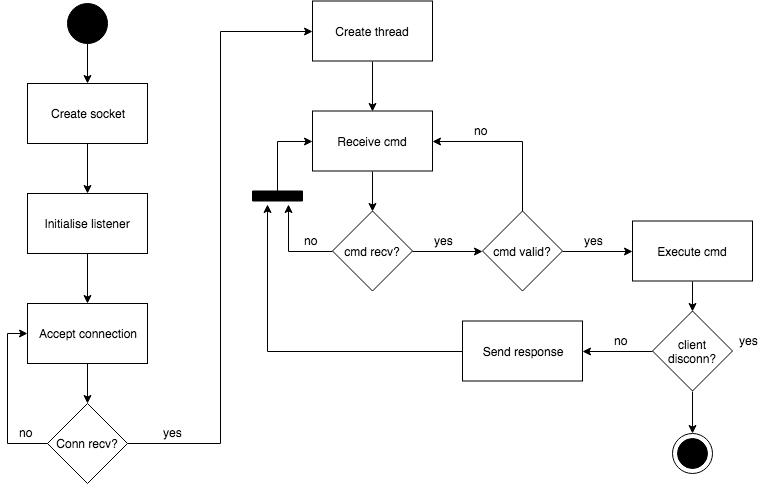
\includegraphics[width=0.9\textwidth]{Server.png}
	\caption{Flow chart depicting the process of server handling connections and client requests}
	\raggedright
	\label{fig:server}	
\end{figure}

\subsection{Client Algorithm}

\begin{figure}[h]
	\centering
	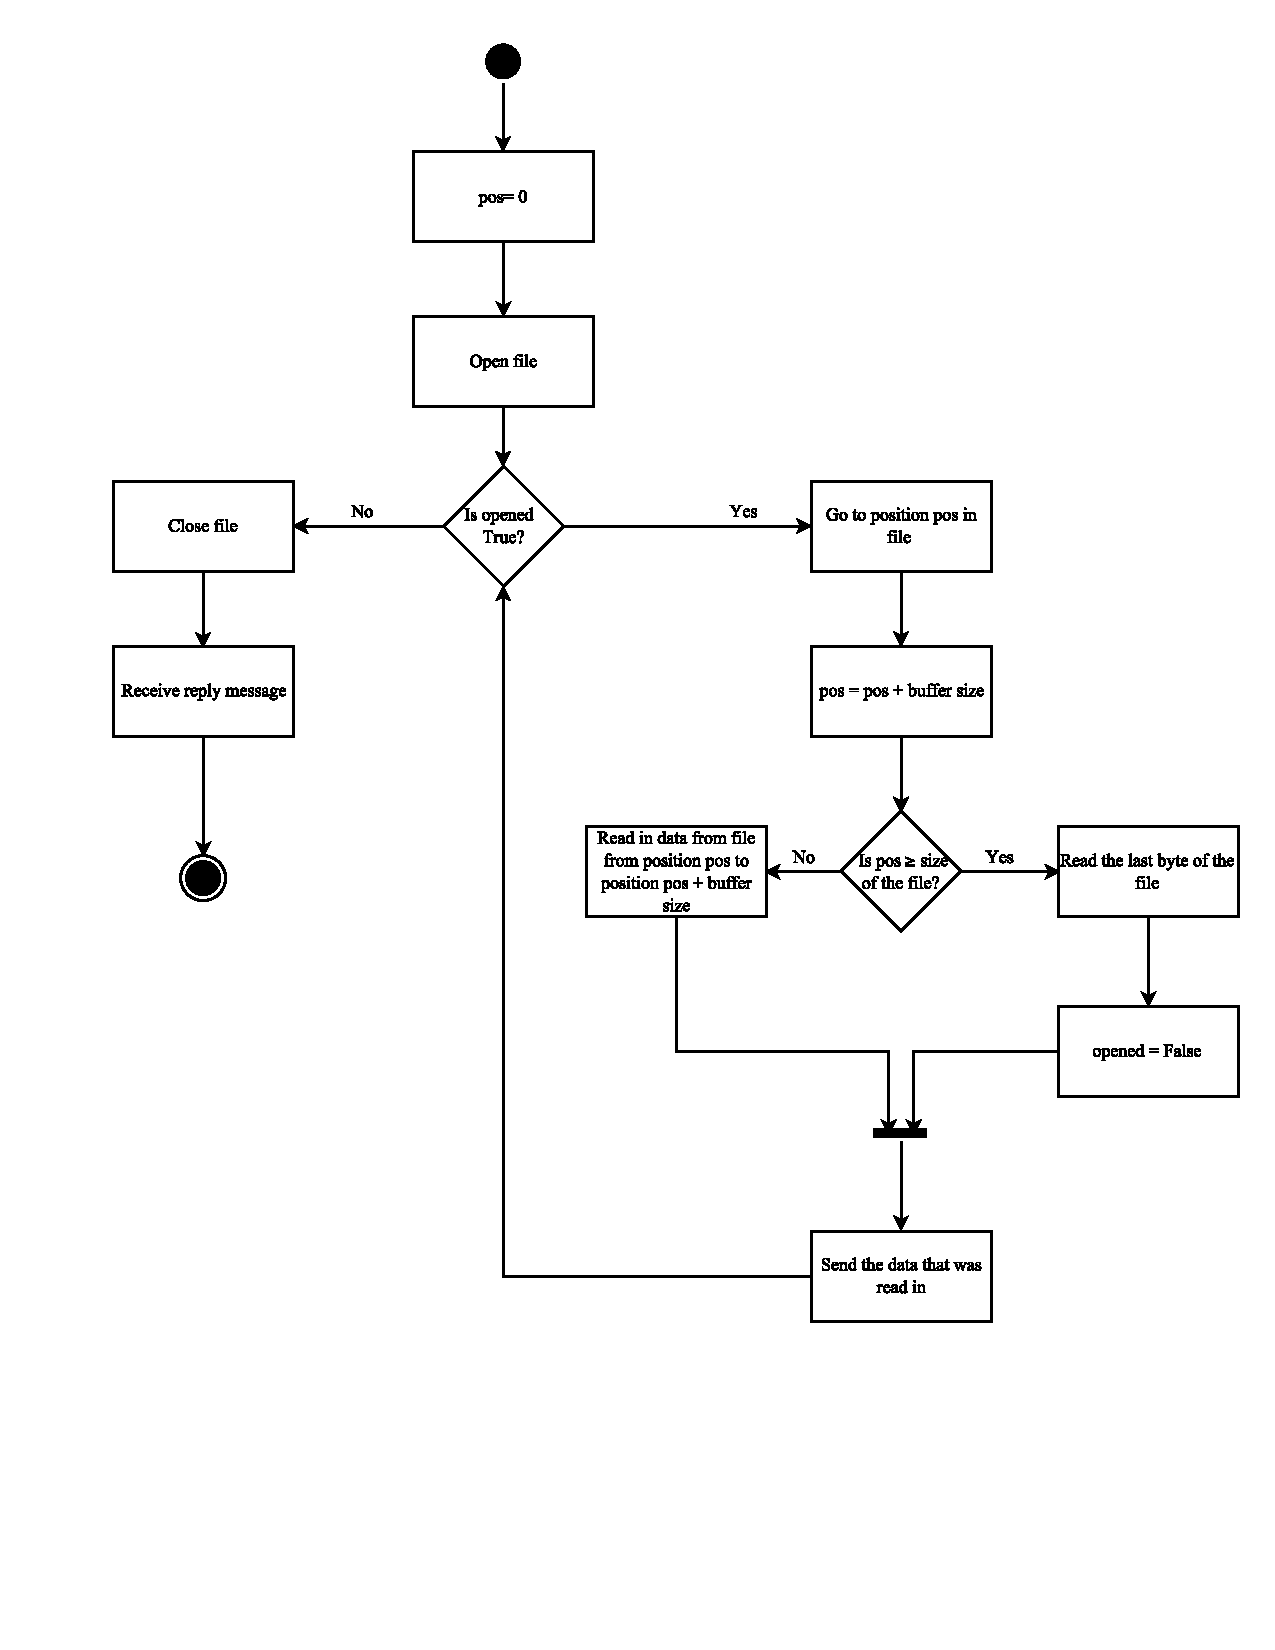
\includegraphics[width=0.9\textwidth]{uploadfile.pdf}
	\caption{Flow chart depicting the process of uploading a file to the server}
	\raggedright
	\label{fig:upload}	
\end{figure}

\newpage
\section{Implemented Commands and Reply Codes}
\setcounter{table}{0}
\renewcommand{\thetable}{B\arabic{table}}

\begin{longtable}{|p{2cm}|p{7cm}|p{7cm}|}
		\caption{Table detailing the implemented commands and reply codes}
		\label{tab:commands} \\
	\hline 
	Command & Description & Reply Code \\ 
	\hline 
	\hline
USER	& Allows the user to input their username in order to be authenticated  &  501 Syntax error in parameters or arguments. 331 User name okay, need password. \\ 
	\hline 
PASS	& Allows the user to input their password for authentication & \makecell[l]{501 Syntax error in parameters or arguments.\\503 Bad sequence of commands. \\230 User logged in, proceed.} \\ 
	\hline 
TYPE	& Its argument is used to specify the file type of the file to be retrieved or stored & \makecell[l]{200 Binary file mode.\\200 Ascii file mode. \\501 Syntax error in parameters or arguments.}\\ 
	\hline 
PASV	& Requests that the server listens on a new data port and waits for a connection & 227 Entering Passive Mode (\textit{IP Address, Port}) \\ 
	\hline 
MODE	& Its argument is used to specify the data transfer type. Only stream transfer mode was implemented & \makecell[l]{200 Stream transfer mode. \\502 Command not implemented. \\501 Syntax error in parameters or arguments.} \\ 
	\hline 
STRU	& Its argument is used to specify the file structure of the file to be retrieved or stored. Only the File type was implemented  & \makecell[l]{200 File Structure = File. \\502 Command not implemented.} \\ 
	\hline 
STAT	& The command causes a status response to be sent over the control connection. The functionality for this command was not implemented & 502 Command not implemented. \\ 
	\hline 
PORT	& The argument specifies the data port to be used in the data connection & 200 Get port. \\ 
	\hline 
LIST & Returns a list of the contents of a directory including permissions. The argument is used to specify the path in which the contents should be returned. If an argument is not provided, a list of the contents of the current working directory is supplied &\makecell[l]{530 User not logged in. \\550 LIST failed Path name not exists. \\150 Here is listing. \\226 List done.}\\ 
	\hline 
NLST & Returns a list of the names of the contents of a directory & \makecell[l]{530 User not logged in. \\550 NLST failed Path name not exists. \\150 Here is listing. \\226 List done.} \\ 
	\hline 
CWD	& Changes the working directory of the server. The argument is used to specify the new working directory.  & \makecell[l]{550 CWD failed. Directory does not exist. \\250 CWD Command successful.} \\ 
	\hline 
PWD	& Returns the current working directory & 257 \textit{Path to current working directory} \\ 
	\hline 
CDUP	& Changes the working directory to the parent of the current directory. & 200 OK. \\ 
	\hline 
DELE	& Deletes a file off the remote host. Its argument is used to specify the file to be deleted & \makecell[l]{530 User not logged in. \\550 DELE failed File \textit{file name} does not exist. \\450 DELE failed delete not allowed. \\250 File deleted.} \\ 
	\hline 
MKD	& Makes a file on the remote host. Its argument specifies the path to the new file and the name of the file to be created & \makecell[l]{530 User not logged in. \\257 Directory created. \\550 MKD failed. Directory "\textit{directory name}" \\already exists.}\\ 
	\hline 
RMD	& Deletes a directory off the remote host. Its argument is used to specify the directory to be deleted & \makecell[l]{530 User not logged in. \\450 Invalid permissions. \\250 Directory deleted.}\\ 
	\hline 
RNFR	& Its argument specifies a file to be renamed & \makecell[l]{550 RNFR failed. File or Directory \textit{file or}\\ \textit{directory name} does not exist. \\350 RNFR successful - awaiting RNTO}\\ 
	\hline 
RNTO	& Its argument specifies the new name of file. The file to be renamed was indicated using the RNFR command prior to calling the RNTO command & \makecell[l]{550 RNTO failed. File or Directory \textit{file or}\\ \textit{directory name} does not exist. \\250 RNTO successful}\\ 
	\hline 
REST	& The argument field represents the checkpoint at which the file transfer is to be restarted.  & 250 File position reset. \\ 
	\hline 
RETR	& This command causes the server to send a copy of a file over the data connection. The argument specifies the name of the file to be downloaded &  \makecell[l]{150 Opening data connection. \\226 Transfer complete.} \\ 
	\hline 
STOR	& This command causes the server to save a copy of a file that is sent over the data connection. The argument specifies the name of the file that is being uploaded &  \makecell[l]{530 STOR failed. User is not logged in. \\150 Opening data connection. \\226 Transfer completed.} \\ 
	\hline 
APPE	& This command causes the server to save a copy of a file that is sent over the data connection. If the file name exists at the path on the server, data is appended to the file. Otherwise, a new file is created &  \makecell[l]{530 APPE failed. User is not logged in. \\150 Opening data connection. \\226 Transfer completed.}\\ 
	\hline 
SYST	& Used to find the server's operating system type & 215 \textit{server operating system} type. \\ 
	\hline 
NOOP	& Prompts a 200 OK response from the server. & 200 OK. \\ 
	\hline 
HELP	& Displays help information &  \\ 
	\hline 
QUIT	& Terminates the control connection between the user and the server &  221 Goodbye.\\ 
	\hline 

\end{longtable}

\newpage
\setcounter{figure}{0} 
\renewcommand{\thefigure}
{C\arabic{figure}}

\section{Results}
This section contains all of the results collected during the testing of the system. This includes Wireshark excerpts and an image of the client GUI.

\subsection{Interaction between the implemented FTP server and client}\label{sec:ourserverourclient}
This section contains images and Wireshark screenshots (\figref{fig:gui} to \figref{fig:logout}) depicting the interaction between the implemented client and server when running on two different hosts within the same network. 

\begin{figure}[h]
	\centering
	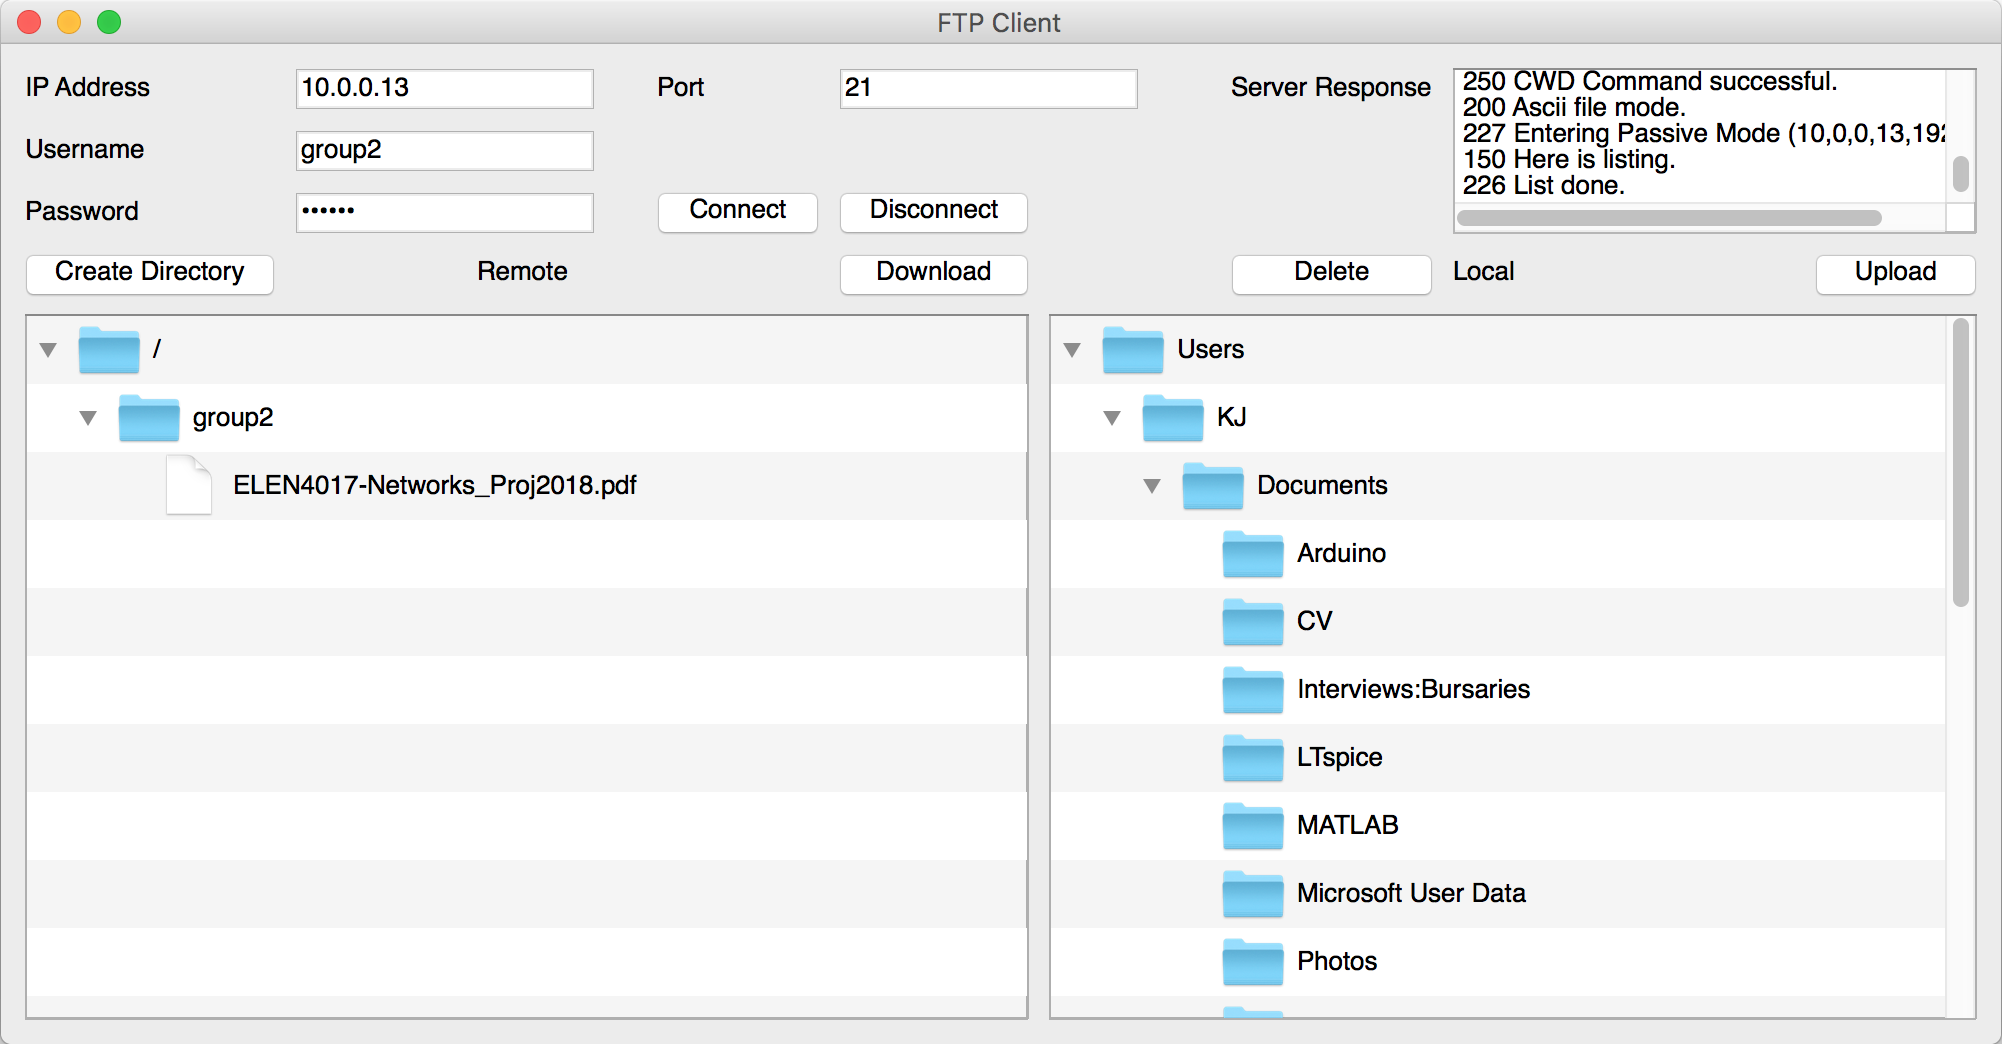
\includegraphics[width=0.9\textwidth]{gui.png}
	\caption{GUI client interacting with the implemented FTP server}
	\raggedright
	\label{fig:gui}	
\end{figure}

\begin{figure}[h]
	\centering
	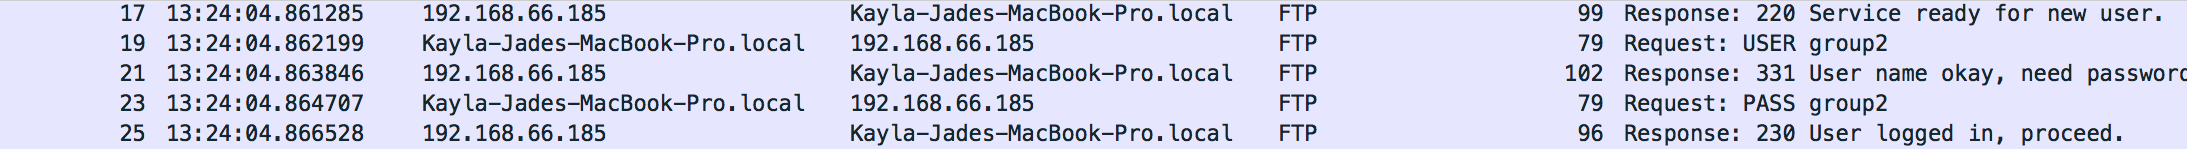
\includegraphics[width=0.9\textwidth]{ourServerLogin.png}
	\caption{FTP commands and replies when logging in}
	\raggedright
	\label{fig:login}	
\end{figure}

\begin{figure}[h]
	\centering
	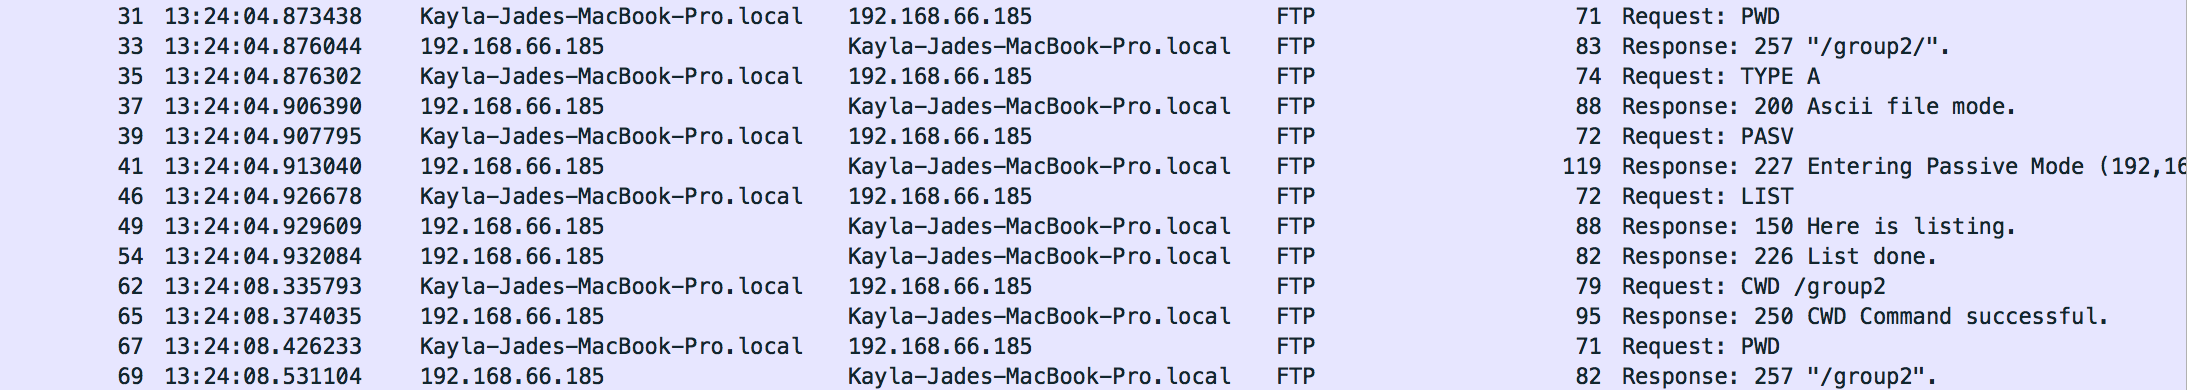
\includegraphics[width=0.9\textwidth]{ourServerNavigate.png}
	\caption{FTP commands and replies when navigating the remote file system}
	\raggedright
	\label{fig:navigate}	
\end{figure}

\begin{figure}[h]
	\centering
	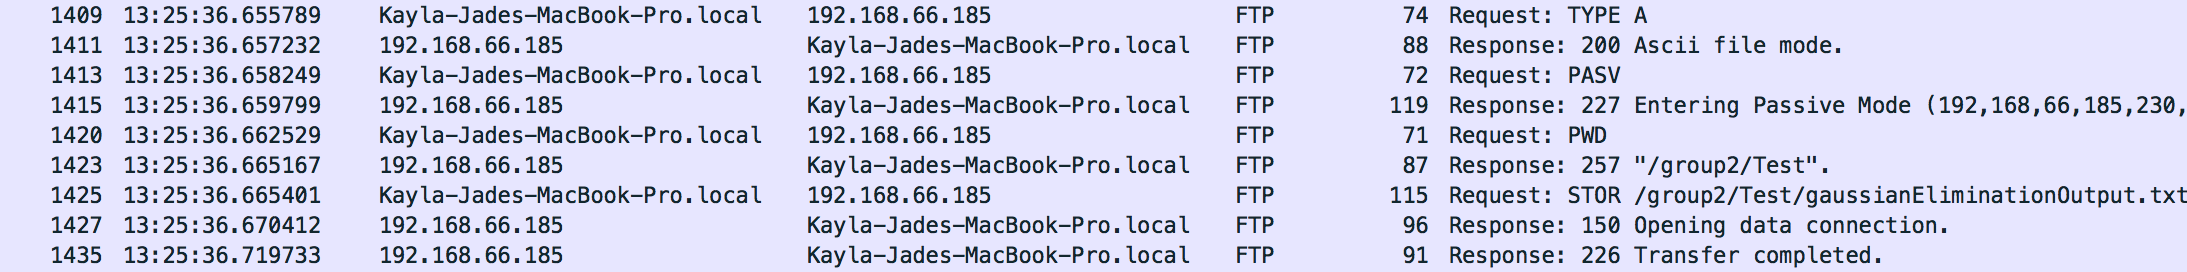
\includegraphics[width=0.9\textwidth]{ourServerUploadText.png}
	\caption{FTP commands and replies when uploading an ASCII type file}
	\raggedright
	\label{fig:textupload}	
\end{figure}

\begin{figure}[h]
	\centering
	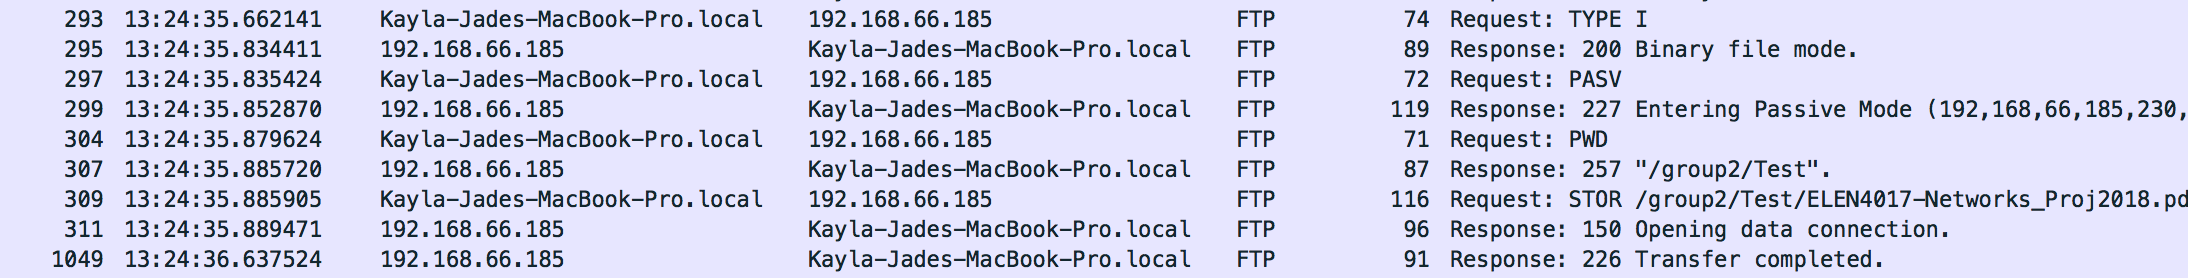
\includegraphics[width=0.9\textwidth]{ourServerUploadPDF.png}
	\caption{FTP commands and replies when uploading an image type file}
	\raggedright
	\label{fig:pdfupload}	
\end{figure}

\begin{figure}[h]
	\centering
	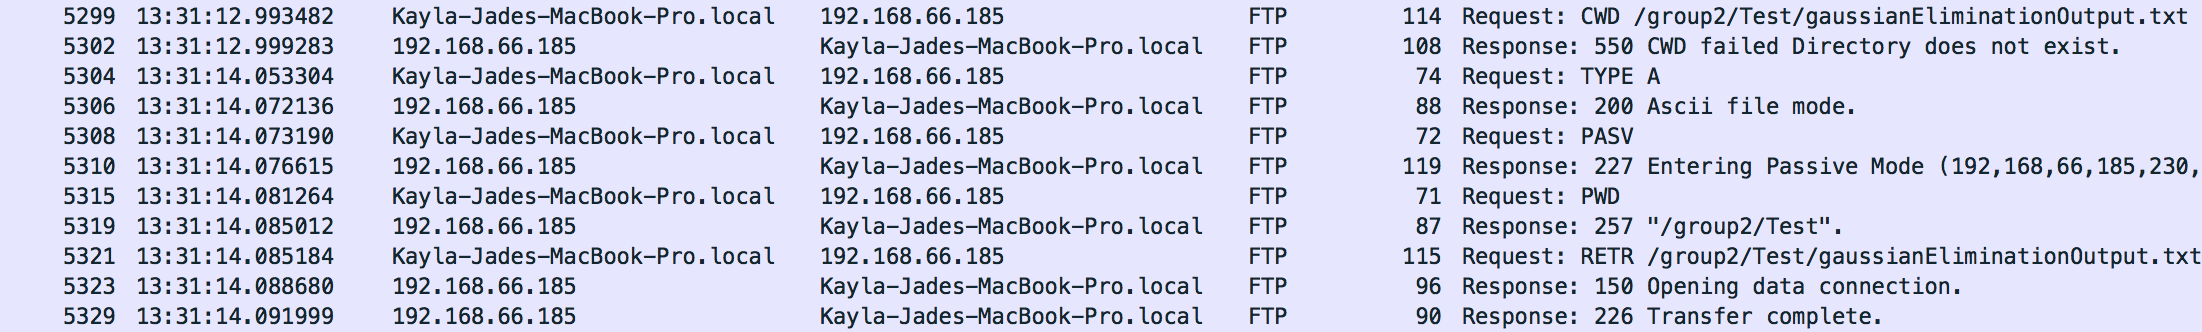
\includegraphics[width=0.9\textwidth]{ourserverDownloadtext.png}
	\caption{FTP commands and replies when downloading an ASCII type file}
	\raggedright
	\label{fig:textdownload}	
\end{figure}

\begin{figure}[h]
	\centering
	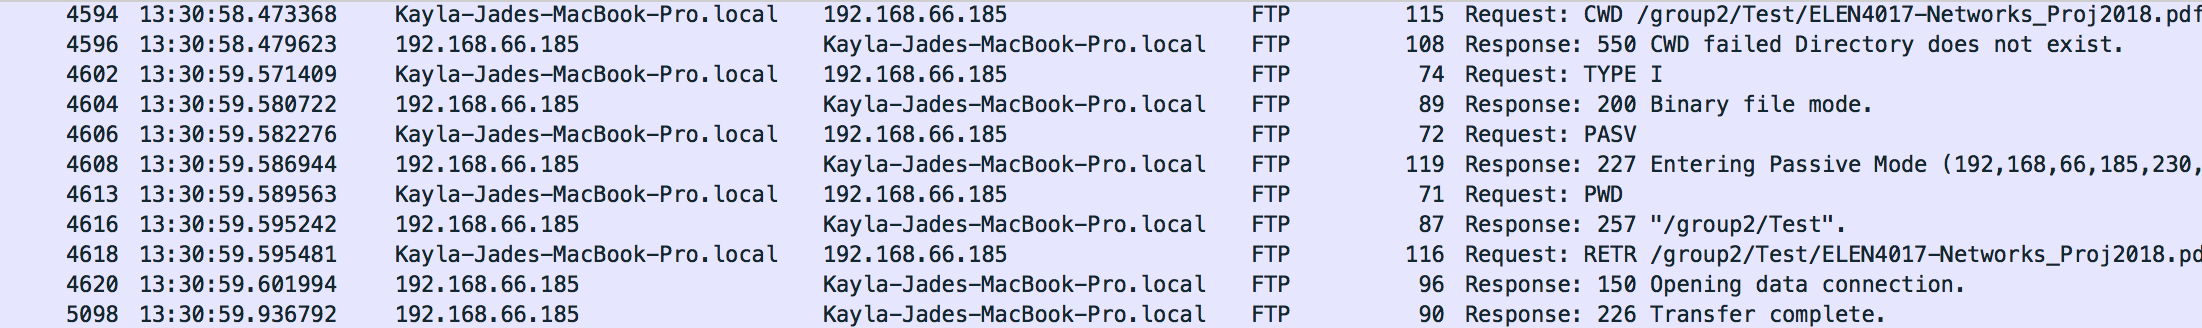
\includegraphics[width=0.9\textwidth]{ourserverDownloadPDF.png}
	\caption{FTP commands and replies when downloading an image type file}
	\raggedright
	\label{fig:pdfdownload}	
\end{figure}

\begin{figure}[h]
	\centering
	
\includegraphics[width=0.9\textwidth]{ourServerMKD.png}
	\caption{FTP commands and replies when creating a directory}
	\raggedright
	\label{fig:makeDirectory}	
\end{figure}

\begin{figure}[h]
	\centering
	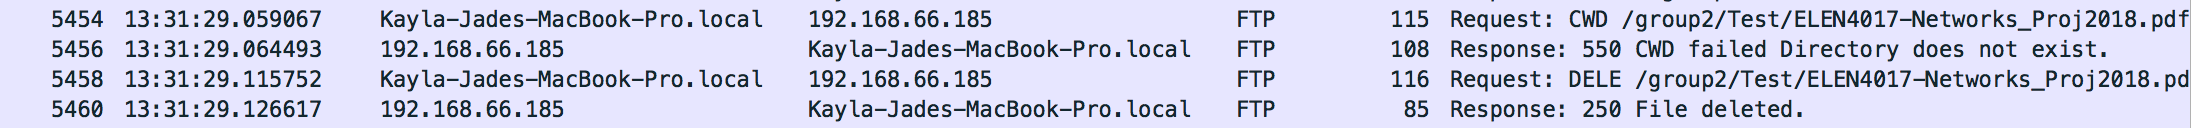
\includegraphics[width=0.9\textwidth]{ourserverDeleteFile.png}
	\caption{FTP commands and replies when deleting a file}
	\raggedright
	\label{fig:delete}	
\end{figure}

\begin{figure}[h]
	\centering
	
\includegraphics[width=0.9\textwidth]{ourserverdeletefolder.png}
	\caption{FTP commands and replies when deleting a directory}
	\raggedright
	\label{fig:deleteFolder}	
\end{figure}

\begin{figure}[h]
	\centering
	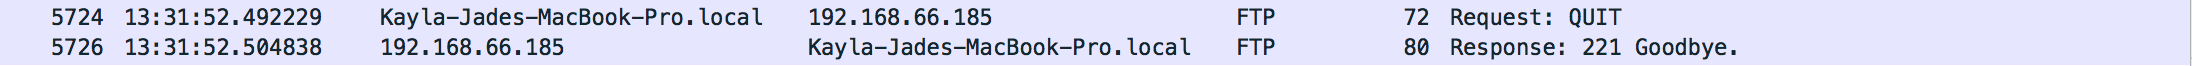
\includegraphics[width=0.9\textwidth]{ourserverquit.png}
	\caption{FTP commands and replies when logging out from the server}
	\raggedright
	\label{fig:logout}	
\end{figure}

\begin{figure}[h]
	\centering
	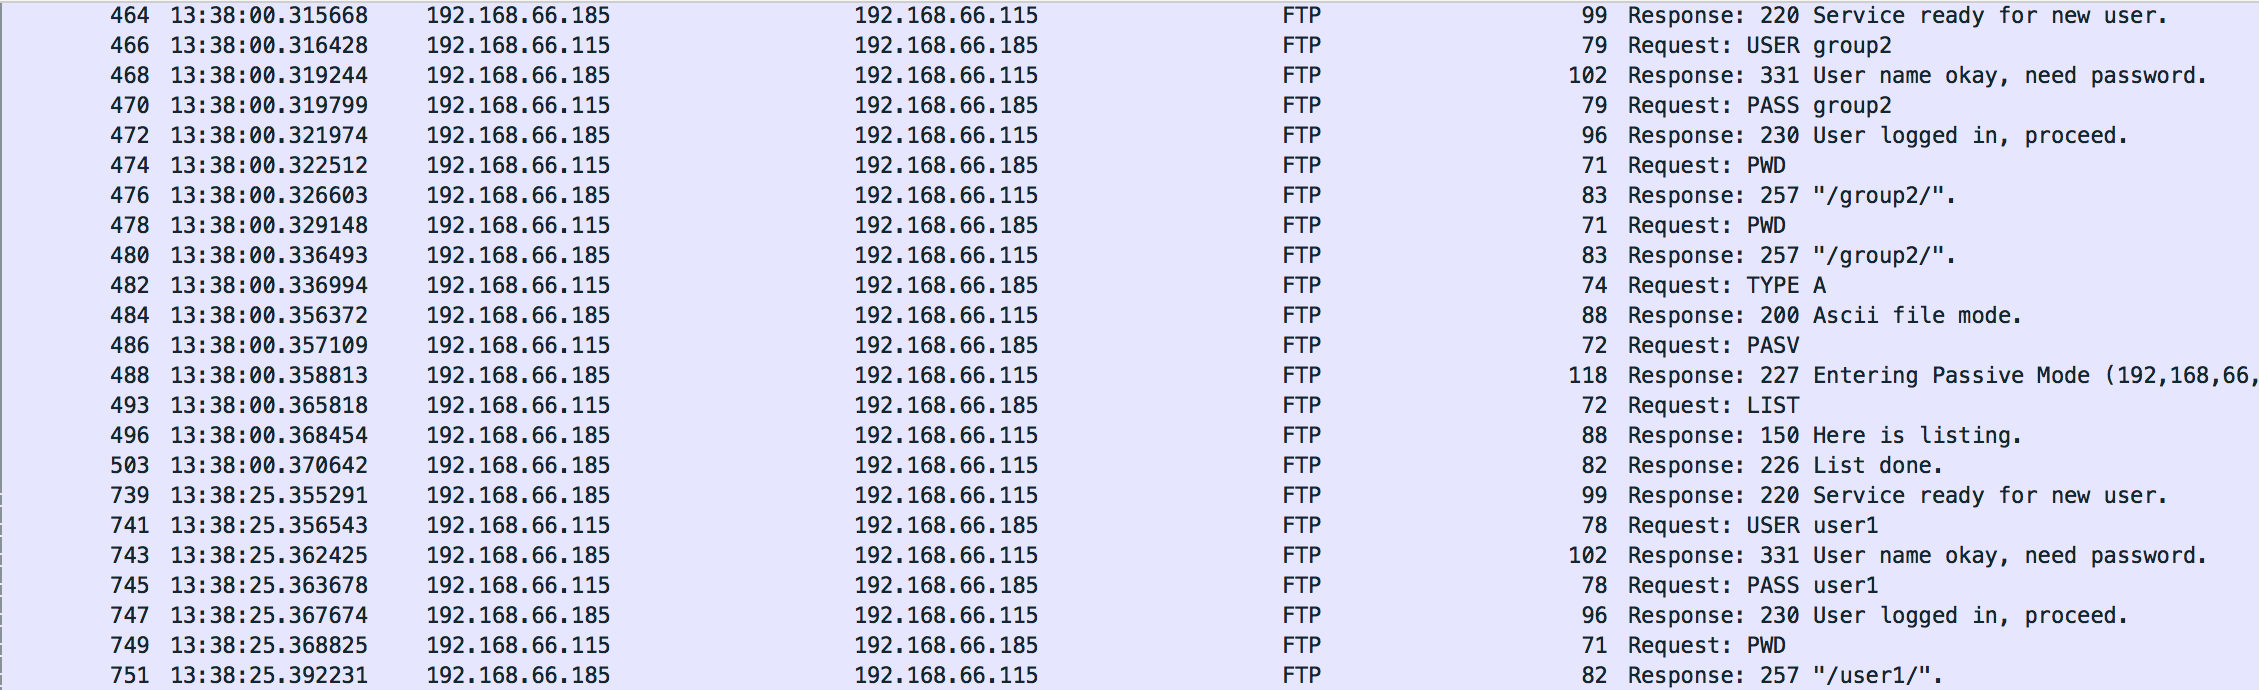
\includegraphics[width=0.9\textwidth]{multipleConnections.png}
	\caption{Multiple clients connected simultaneously to the FTP server}
	\raggedright
	\label{fig:multiple}	
\end{figure}

\begin{figure}[h]
	\centering
	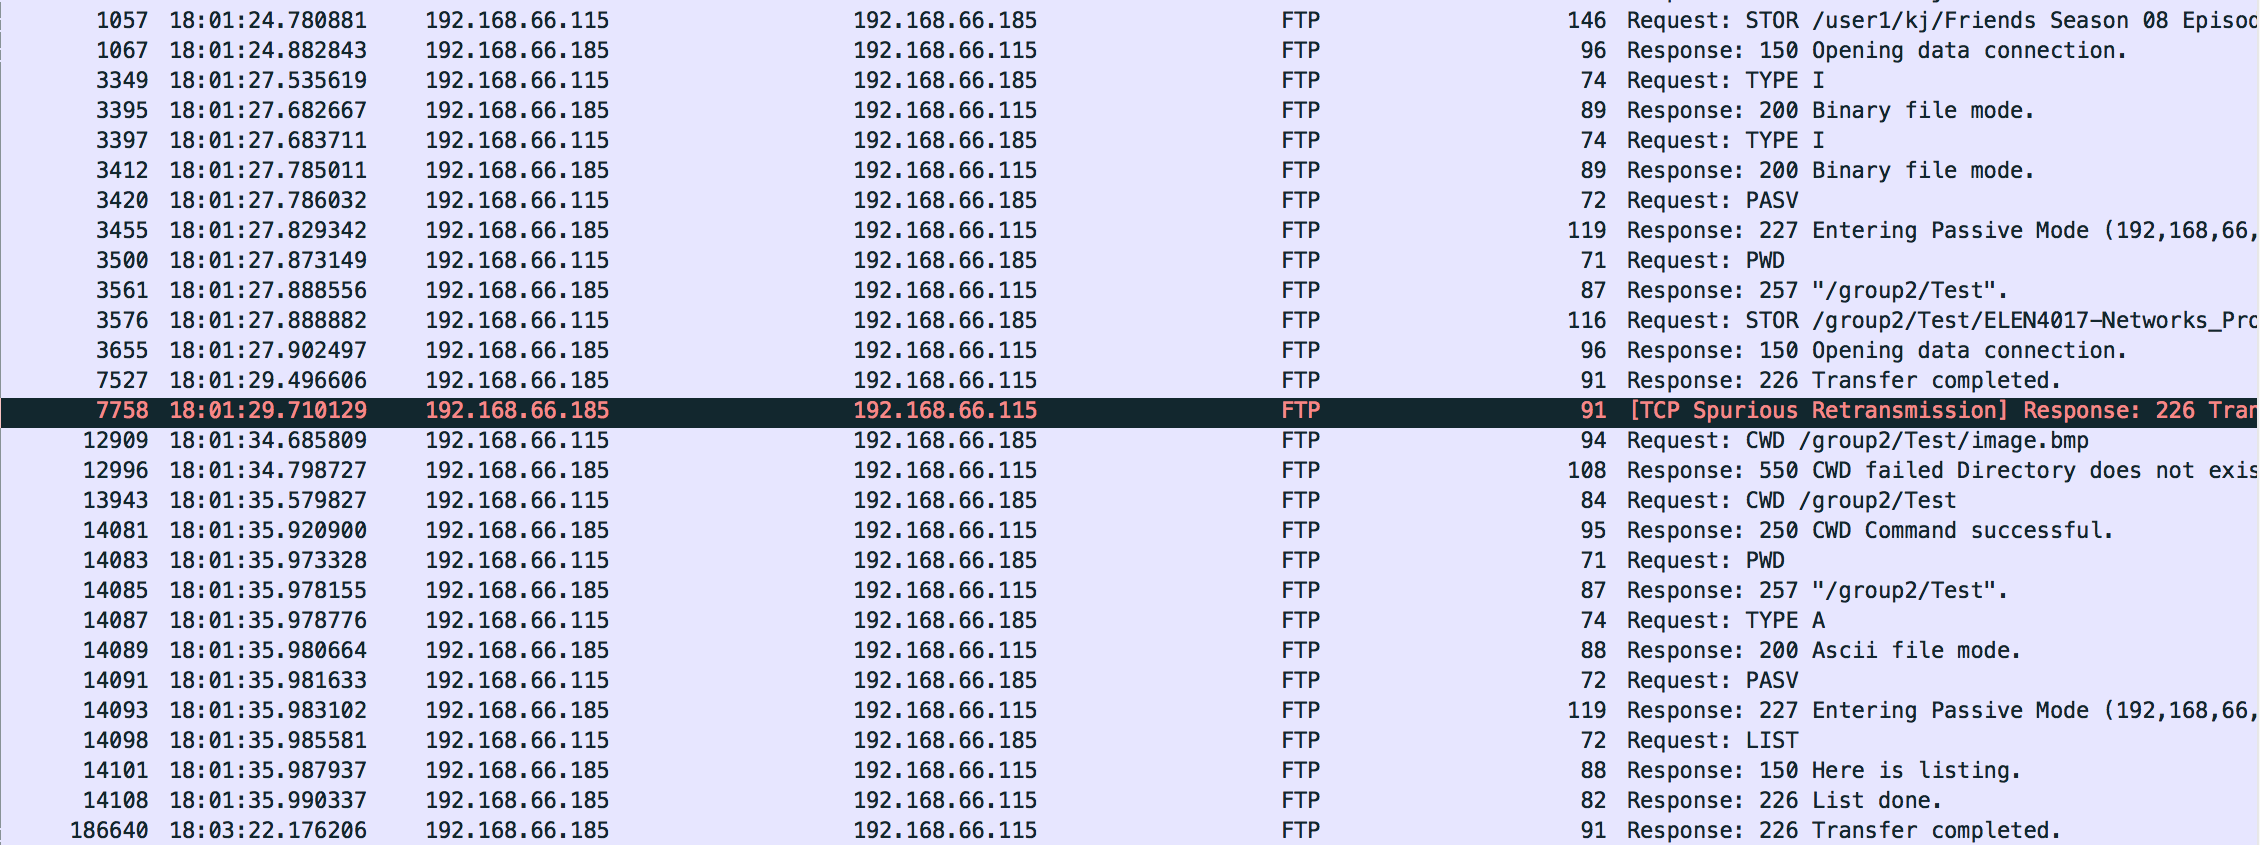
\includegraphics[width=0.9\textwidth]{multipleUpload.png}
	\caption{Multiple clients simultaneously uploading files to the FTP server}
	\raggedright
	\label{fig:multipleUpload}	
\end{figure}

\subsection{Interaction between a standard FTP server and the implemented client} \label{sec:ourClientWitsServer}

Wireshark screenshots (\figref{fig:loginWits} to \figref{fig:logoutWits}) depicting the interaction between the created client and the standard FTP server are given in this section.

\begin{figure}[h]
	\centering
	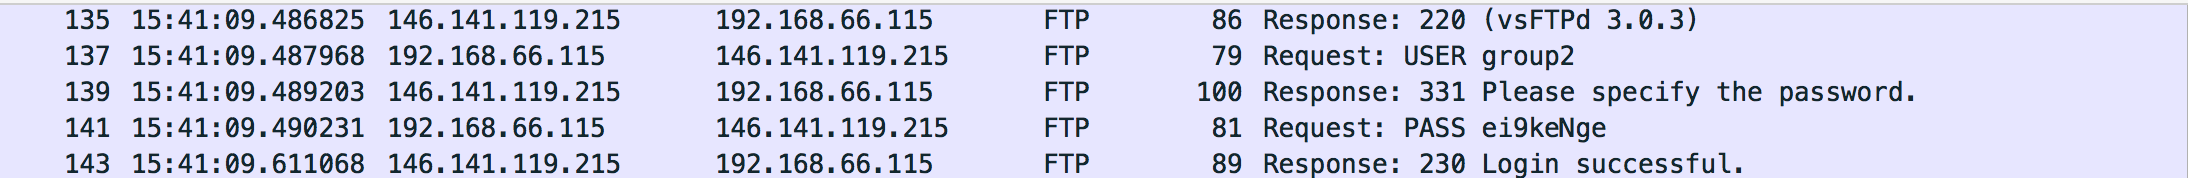
\includegraphics[width=1\textwidth]{loginWits.png}
	\caption{FTP commands and replies when logging in}
	\raggedright
	\label{fig:loginWits}	
\end{figure}

\begin{figure}[h]
	\centering
	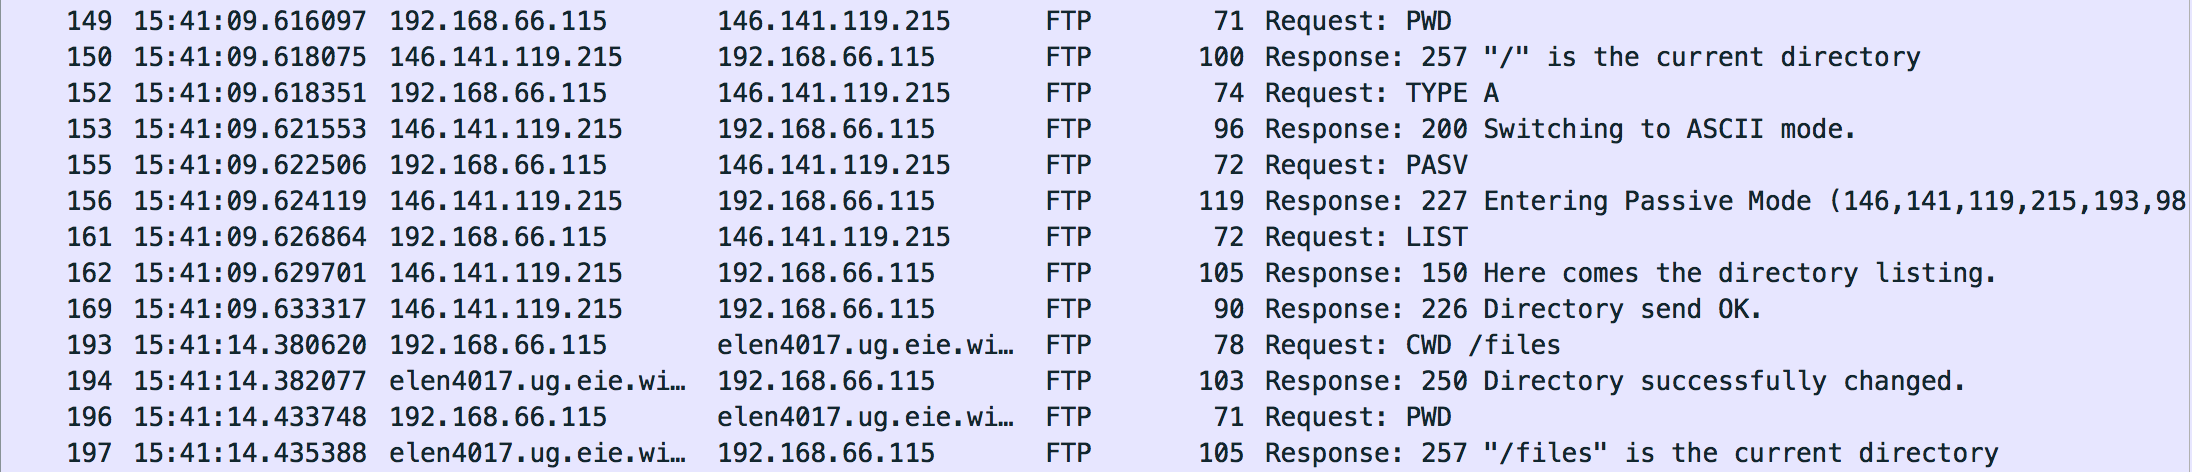
\includegraphics[width=1\textwidth]{navigateWits.png}
	\caption{FTP commands and replies when navigating the remote file system}
	\raggedright
	\label{fig:navigateWits}	
\end{figure}

\begin{figure}[h]
	\centering
	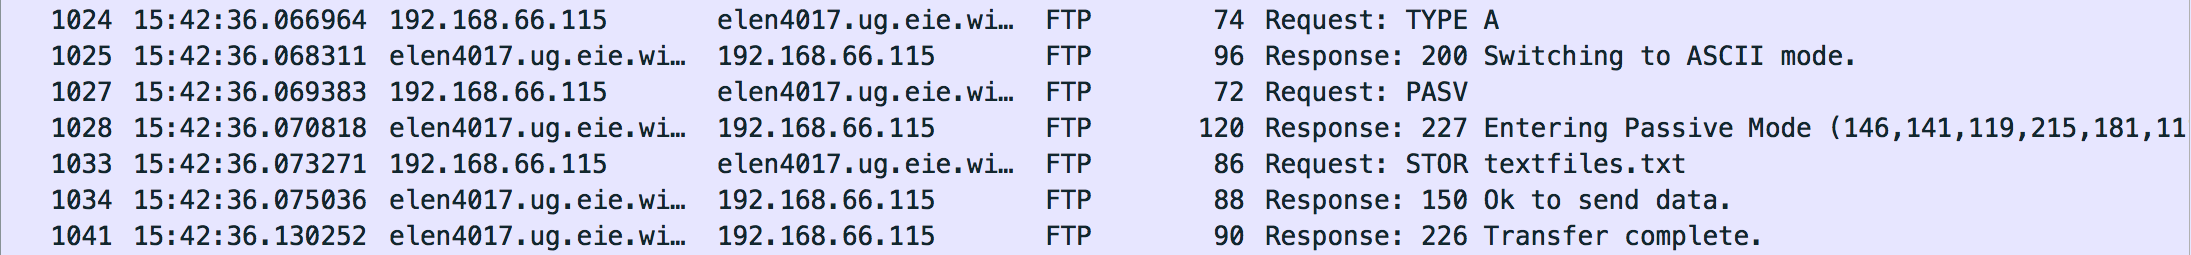
\includegraphics[width=1\textwidth]{textUploadWits.png}
	\caption{FTP commands and replies when uploading an ASCII type file}
	\raggedright
	\label{fig:textUploadWits}	
\end{figure}

\begin{figure}[h]
	\centering
	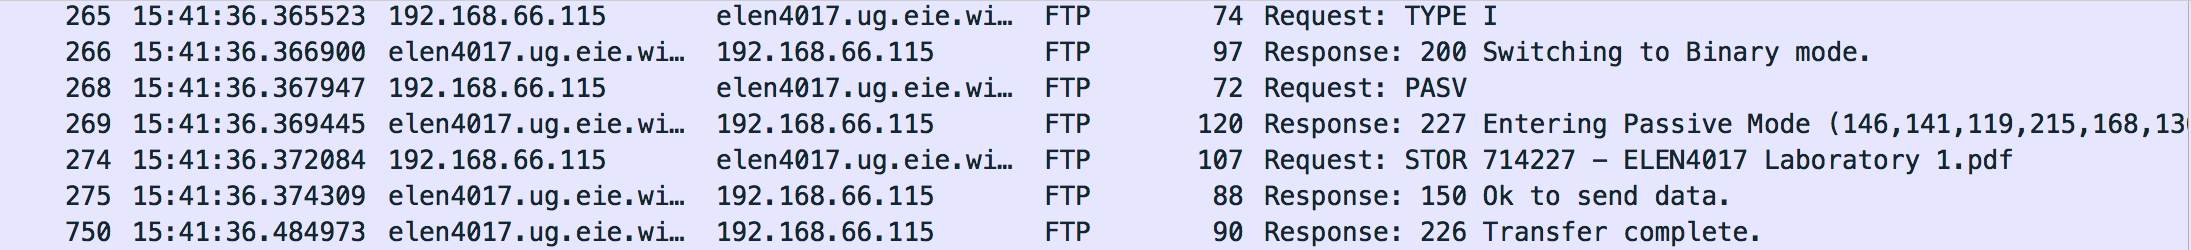
\includegraphics[width=1\textwidth]{binaryUploadWits.png}
	\caption{FTP commands and replies when uploading an image type file}
	\raggedright
	\label{fig:binaryUploadWits}	
\end{figure}

\begin{figure}[h]
	\centering
	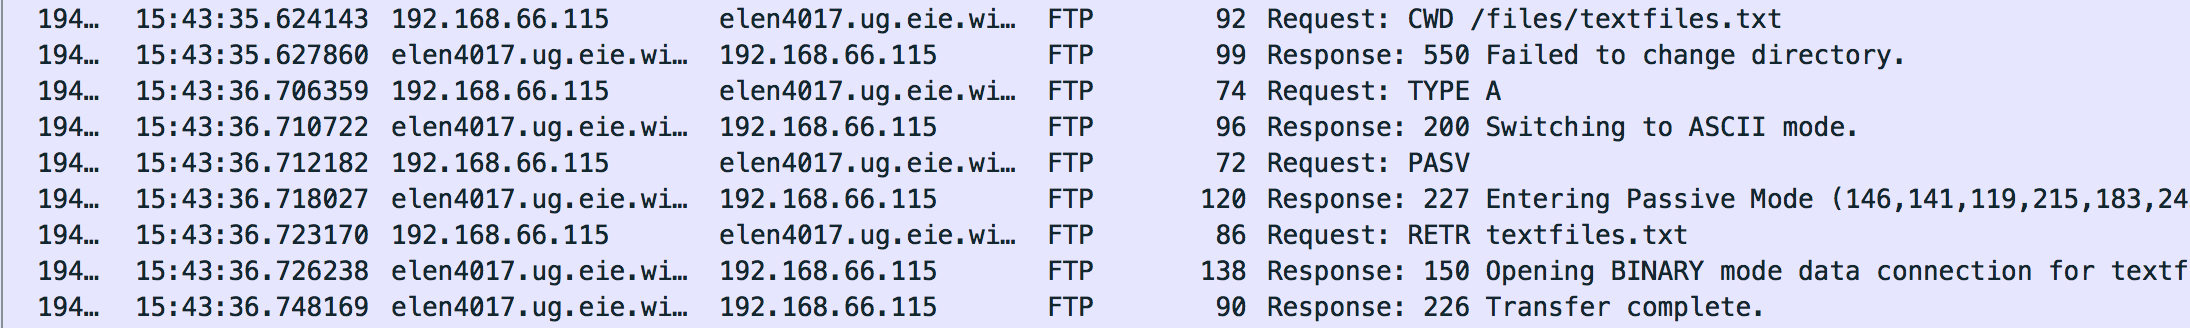
\includegraphics[width=1\textwidth]{downloadTextWits.png}
	\caption{FTP commands and replies when downloading an ASCII type file}
	\raggedright
	\label{fig:textDownloadWits}	
\end{figure}

\begin{figure}[h]
	\centering
	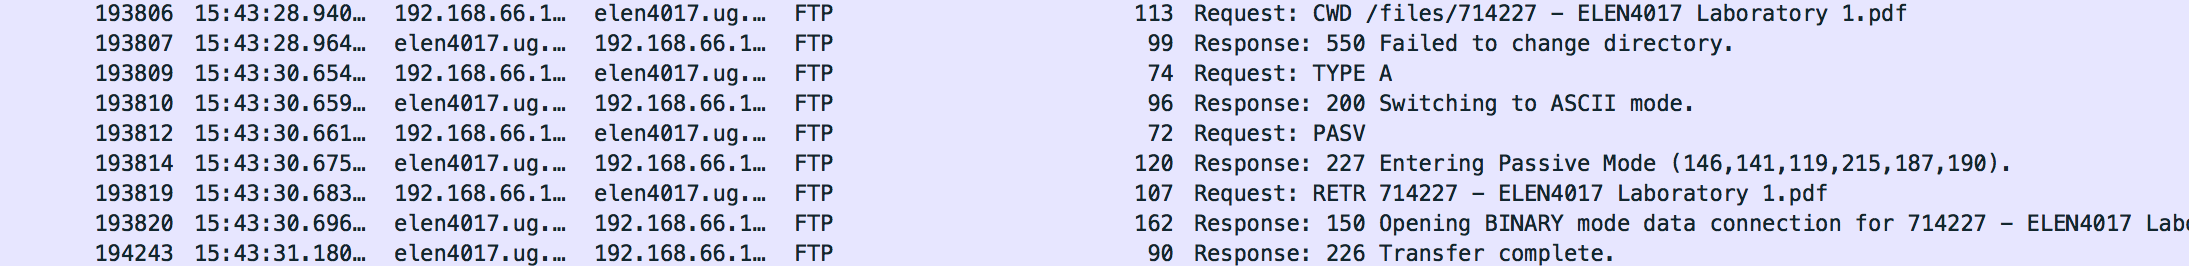
\includegraphics[width=1\textwidth]{downloadImageWits.png}
	\caption{FTP commands and replies when downloading an image type file}
	\raggedright
	\label{fig:binaryDownloadWits}	
\end{figure}

\begin{figure}[h]
	\centering
	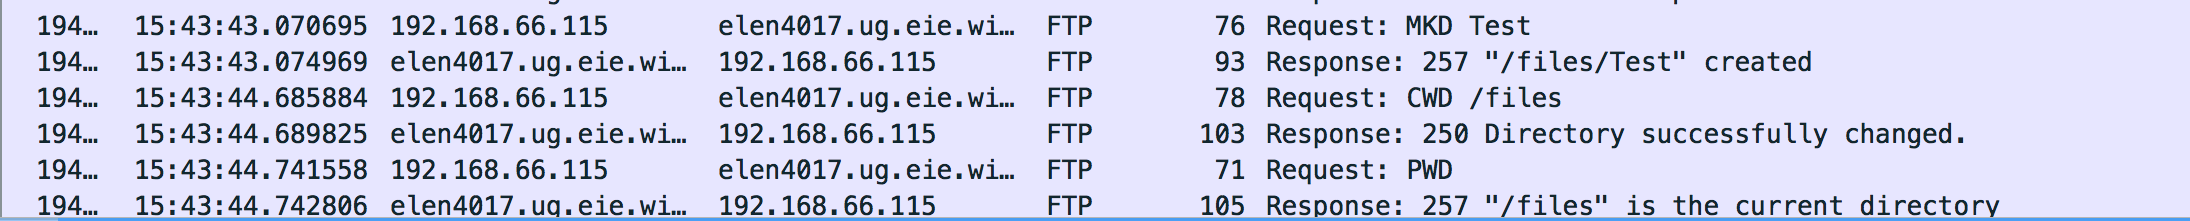
\includegraphics[width=1\textwidth]{makeDirectoryWits.png}
	\caption{FTP commands and replies when creating a directory}
	\raggedright
	\label{fig:makeDirectoryWits}	
\end{figure}

\begin{figure}[h]
	\centering
	
\includegraphics[width=1\textwidth]{deleteDirWits.png}
	\caption{FTP commands and replies when deleting a directory}
	\raggedright
	\label{fig:deleteDirWits}	
\end{figure}

\begin{figure}[h]
	\centering
	
\includegraphics[width=1\textwidth]{deleteFileWits.png}
	\caption{FTP commands and replies when deleting a file}
	\raggedright
	\label{fig:deleteFileWits}	
\end{figure}

\begin{figure}[h]
	\centering
	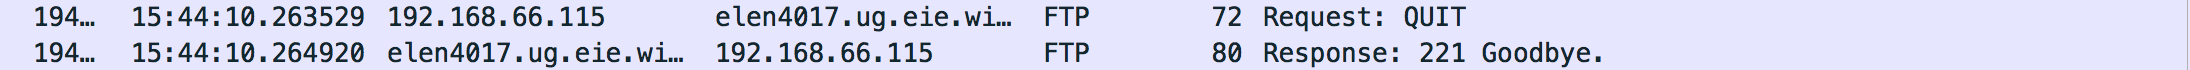
\includegraphics[width=1\textwidth]{logoutWits.png}
	\caption{FTP commands and replies when logging out from the server}
	\raggedright
	\label{fig:logoutWits}	
\end{figure}

\subsection{Interaction between the implemented FTP server and a standard FTP client} \label{sec:ourserverstandardclient}
This section contains Wireshark excerpts depicting the interaction between the server and a standard client when running on two different hosts within the same network. The images for this section are found in \figref{fig:loginclient} to \figref{fig:error}.

\begin{figure}[h]
	\centering
	
\includegraphics[width=1\textwidth]{theirclientLogin.png}
	\caption{FTP commands and replies when logging in}
	\raggedright
	\label{fig:loginclient}	
\end{figure}

\begin{figure}[h]
	\centering
	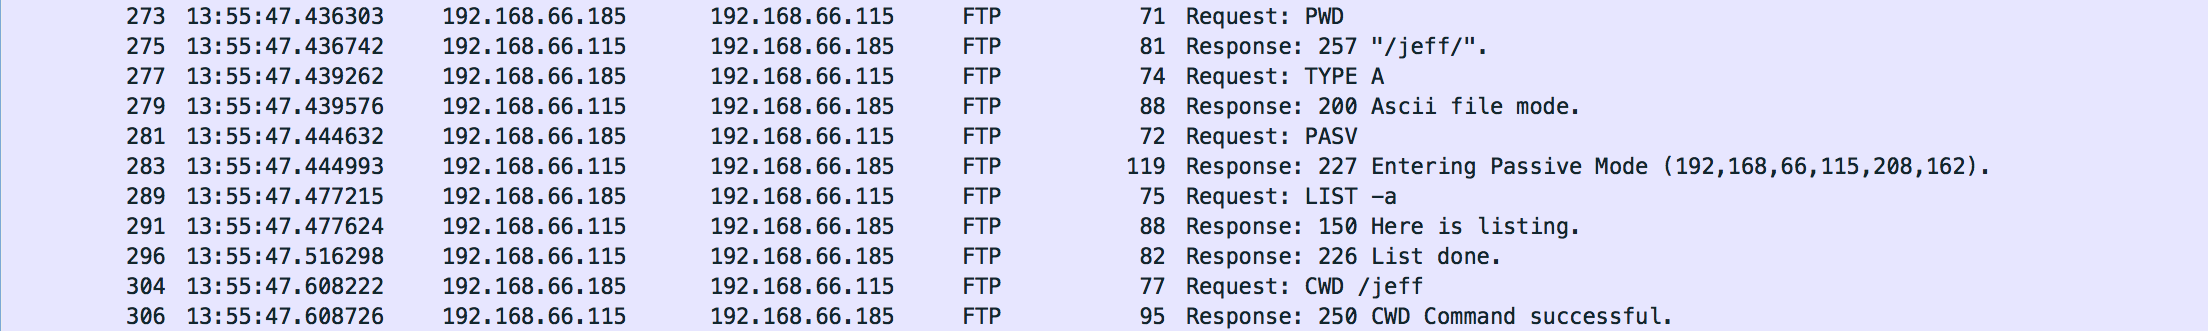
\includegraphics[width=1\textwidth]{theirclientnavigate.png}
	\caption{FTP commands and replies when navigating the remote file system}
	\raggedright
	\label{fig:navigateclient}	
\end{figure}


\begin{figure}[h]
	\centering
	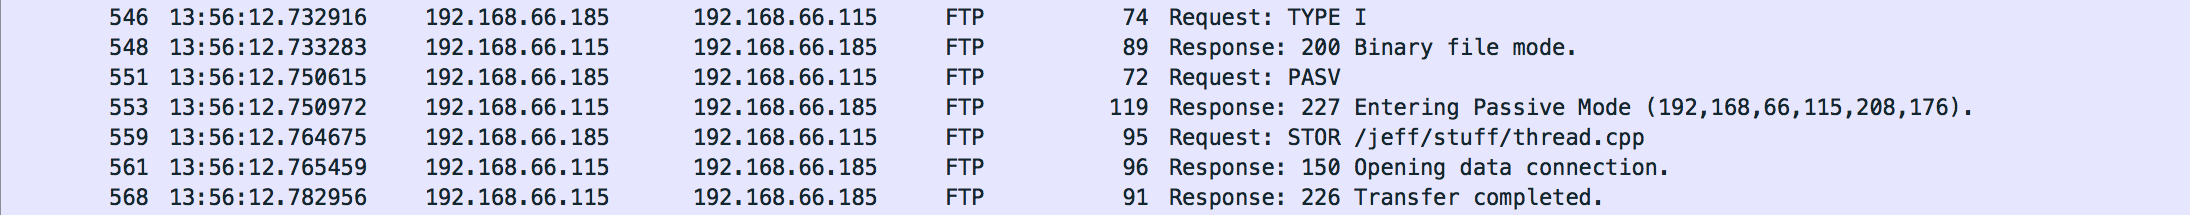
\includegraphics[width=1\textwidth]{theirclientupload.png}
	\caption{FTP commands and replies when uploading an image type file}
	\raggedright
	\label{fig:binaryUploadclient}	
\end{figure}

\begin{figure}[h]
	\centering
	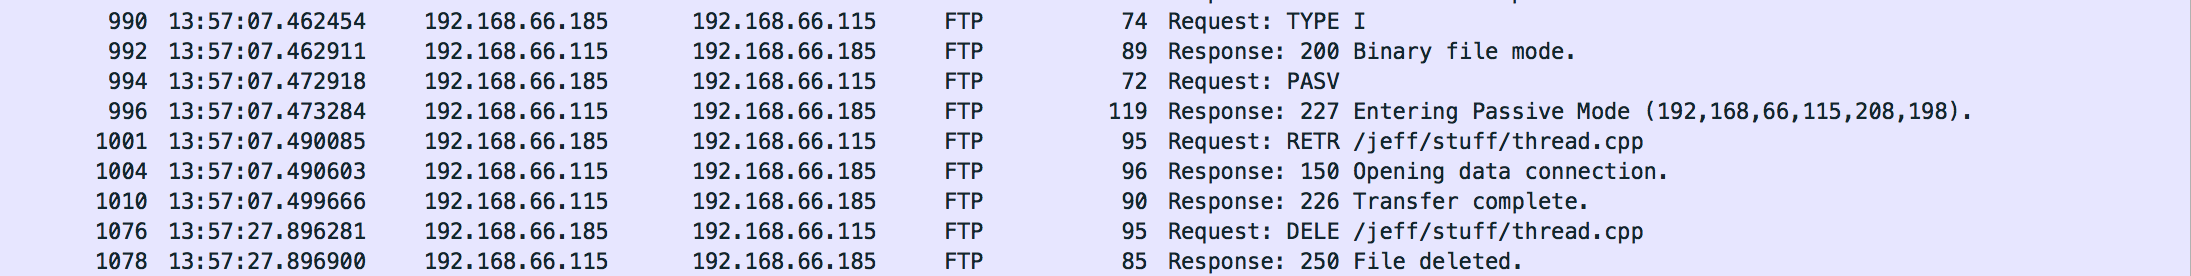
\includegraphics[width=1\textwidth]{theirclientdeleteanddownload.png}
	\caption{FTP commands and replies when downloading an image type file and deleting a file}
	\raggedright
	\label{fig:binaryDownloadclient}	
\end{figure}

\begin{figure}[h]
	\centering
	
\includegraphics[width=1\textwidth]{theirclientMKD.png}
	\caption{FTP commands and replies when creating a directory}
	\raggedright
	\label{fig:makeDirectoryclient}	
\end{figure}

\begin{figure}[h]
	\centering
	
\includegraphics[width=1\textwidth]{theirclientRMD.png}
	\caption{FTP commands and replies when deleting a directory}
	\raggedright
	\label{fig:deleteDirclient}	
\end{figure}

\begin{figure}[h]
	\centering
	
\includegraphics[width=1\textwidth]{theirclientCommandNotKnown.png}
	\caption{FTP commands and replies when an unimplemented command is called}
	\raggedright
	\label{fig:error}	
\end{figure}

\end{appendix}

\end{document}

" vim: ts=4
" vim: tw=78
" vim: autoindent
" vim: shiftwidth=4